\section{Case Studies}
\label{sec:4:case-studies}

In this section, we present several case studies of how the transaction throughput on the three blockchains is used in practice,  for both legitimate and less legitimate purposes.

\subsection{Malicious Transactions on EOSIO}
\label{sec:eoscase}
\point{Exchange Wash-trading}
We investigate WhaleEx, which claims to be the largest decentralized exchange~(DEX) on EOSIO in terms of daily active users~\cite{WhaleEx2020}.
As shown in~\autoref{tab:eos-top-applications}, the most frequently-used action of the WhaleEx contract are \texttt{verifytrade2} and \texttt{verifytrade3}, with a combined total of~\empirical{9,437,393} calls over the seven months observational period, which corresponds to approximately \empirical{one action every two seconds}. These actions are executed when a buy offer and a sell offer match each other and signal a settled trade.

% Therefore, it is also the action we are the most interested in, as this is what we need to analyze to understand the movement of assets.

%Therefore, we start by analysing these accounts and look for patterns which could correspond to wash-trading.

Firstly, and most obviously, we notice that in more than~\empirical{75\%} of the trades, the buyer and the seller are \emph{the same}.
This means that no asset is transferred at the end of the action.
Furthermore, the transaction fees for both the buyer and the seller are~0, which means that such a transaction is achieving absolutely nothing else than \emph{artificially} increasing the service statistics, i.e. wash-trading.

Further investigation reveals that accounts involved in the trades that are signalled by either \texttt{verifytrade2} or \texttt{verifytrade3} are highly concentrated: the top~5 accounts, as either a ``seller'' or a ``buyer'', are associated with over~\empirical{78\%} of the trades.
We compute the percentage of such transactions for the top~5 accounts and find that each of these accounts acts simultaneously as both seller and buyer in more than~\empirical{88\%} of the transactions they are associated with.
This means that the \emph{vast majority} of transactions of the top~5 accounts represent wash-trading.

Next, we analyse the total amount of funds that have been moved, i.e. the difference between the total amount of cryptocurrency sent and received by the same account.
For the most active account, we find that only~\empirical{one} of the~\empirical{4} currencies has a balance change of over~\empirical{0.3\%}.
The second most frequently used account has a similar transaction pattern, with only \empirical{2} out of the~\empirical{32} currencies traded showing a balance change larger than~\empirical{0.6\%}.
The rest of the top accounts all follow a very similar trend, with almost all the traded currencies having almost the same sent and received amounts.

% \point{Summary}
% Overall, we conclude that although a lot of traffic is generated by this exchange, the vast majority is generated to \emph{artificially increase the trading volume} of this exchange. 
% A recurring pattern for such transactions is that they have the same buyer and seller, and both pay no transaction fee, resulting in no state change.

\point{Boomerang transactions}
As shown in~\autoref{fig:eos-throughput-time}, there was a very sharp increase in activity on EOSIO after November 1,~2019. After investigating, we find that this increase is due to the airdrop of a new coin called~\coin{EIDOS}~\cite{Enumivo2019}.

The token distribution works as follows: Users send any amount of \coin{EOS} to the EIDOS contract address, the EIDOS contract sends the \coin{EOS} amount back to the sender and also sends 0.01\% of the \coin{EIDOS} tokens it holds. This creates a ``boomerang'' transaction for the \coin{EOS} token and a transaction to send the \coin{EIDOS} token. The tokens can then be traded for \coin{USDT} (Tether) which can in turn be converted to other currencies. There are no transaction fees on EOSIO and users can execute transactions freely within the limits of their rented CPU capacity. Therefore, this scheme incentivises users with idle CPU resources on EOSIO to send transactions to this address, creating a large increase in the number of transactions.

Soon after the launch of this coin, the price of CPU usage on EOSIO spiked by~10,000\% and the network entered a congestion mode.
In normal mode, users can consume more CPU than they staked for, but when the network is in congestion mode, they can only consume the amount staked. Although this is how the network is supposed to behave, it is problematic if it lasts for a non-negligible period. For example, \coin{EOS} is used for games where many users make a small number of transactions without staking CPU. When the network enters congestion mode for a long period, these users cannot continue to play unless they actively stake \coin{EOS} for CPU.
This has caused some services to threaten with their migration to another blockchain~\cite{EarnBet2019EOSNotice}.

The coin seems to be operated by an entity called Enumivo but there is very scarce information about what service it provides. Given the very hostile tone in communications\footnote{\url{https://twitter.com/enumivo/status/1193353931797057536}}, it is likely that the creator indeed intended to congest the EOSIO network. Furthermore, the entity behind the \coin{EIDOS} token seems to be willing to launch a ``sidechain'' of EOSIO~\cite{yas-network}.

\begin{figure*}[tb]
	\centering
	\begin{subfigure}{0.323\textwidth}
		\centering
		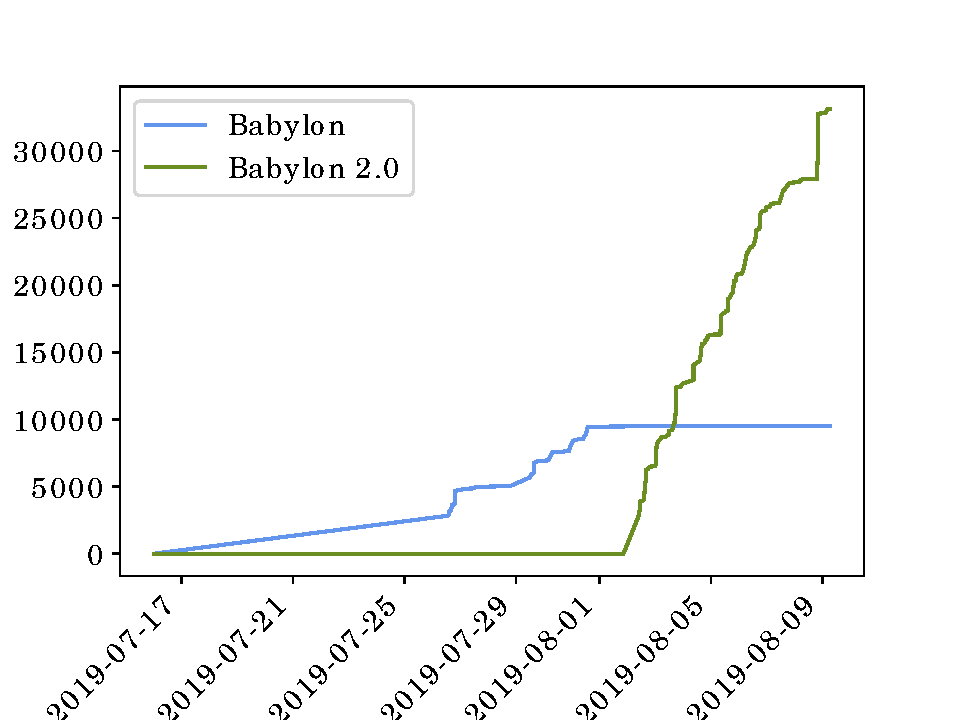
\includegraphics[width=\columnwidth]{./4-transactions-security/figures/babylon-proposals.pdf}
		\caption{Proposal period}
	\end{subfigure}
	%
	\begin{subfigure}{0.323\textwidth}
		\centering
		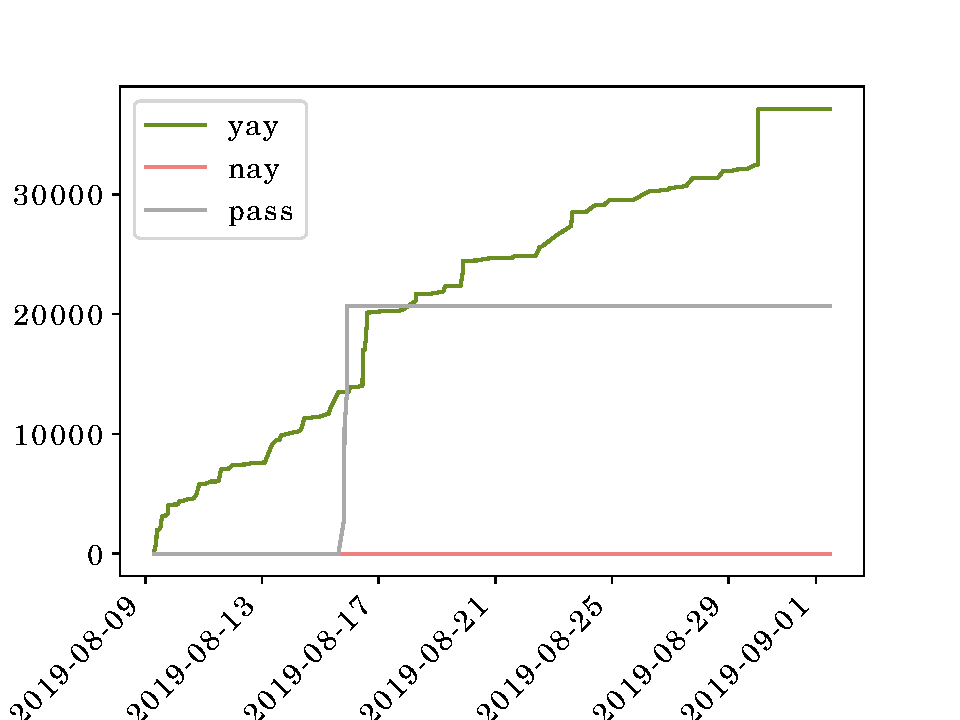
\includegraphics[width=\columnwidth]{./4-transactions-security/figures/babylon-exploration.pdf}
		\caption{Exploration period}
	\end{subfigure}
	%
	\begin{subfigure}{0.323\textwidth}
		\centering
		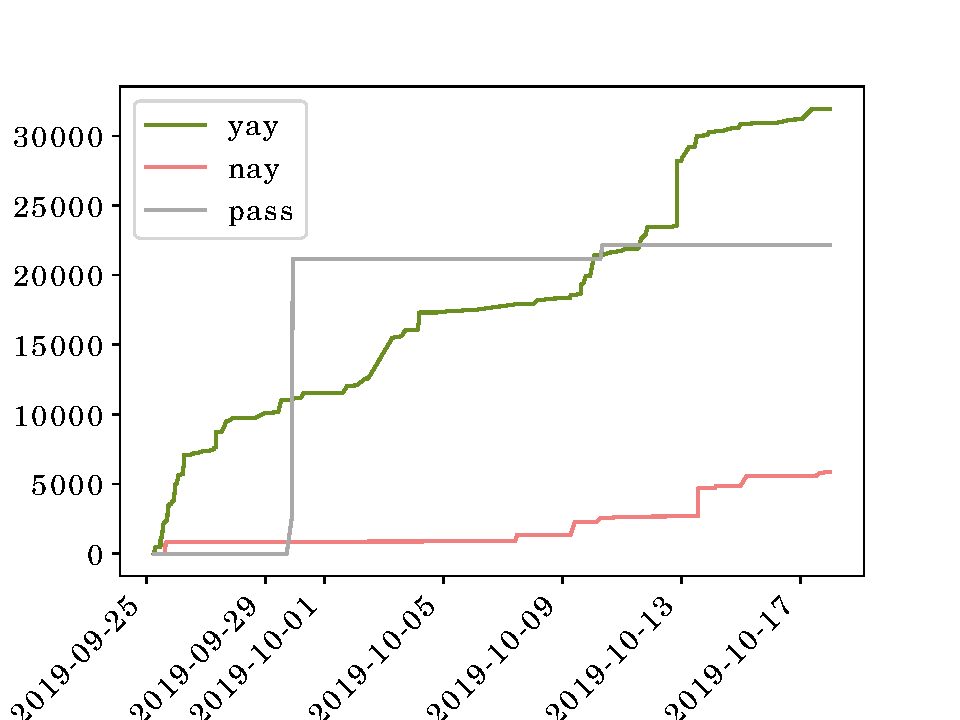
\includegraphics[width=\columnwidth]{./4-transactions-security/figures/babylon-promotion.pdf}
		\caption{Promotion period}
	\end{subfigure}
	\caption{Tezos Babylon on-chain amendment voting process.}
	\label{fig:tezos-votes}
\end{figure*}

\point{Summary}
One of the major selling points of EOSIO is its absence of transaction fees for most users. Although this provides advantages for users, it can also result in spamming behaviours, as observed in this section. The fee-free transaction environment encourages market manipulation such as the WhaleEx wash-trading; moreover, it has also back-fired with the \coin{EIDOS} token, as the network had to enter congestion mode and users have to stake an amount much higher than transaction fees in the Bitcoin network~\cite{EarnBet2019EOSNotice}.


\subsection{Governance Transactions on Tezos}
One of the main particularities of Tezos, compared to other blockchains, is its on-chain governance and self-amendment abilities. Given that only~\emph{bakers} are allowed to send such transactions and that they can only perform a limited number of actions within a certain time frame, governance-related transactions represent only a very small fraction of the total number of transactions: merely~\empirical{604} within our observation period. However, given that this type of transaction is rather unique and has, to the best of our knowledge, not been researched before, we analyze how the different phases of the governance process are executed in practice.

\point{Tezos voting periods}
Tezos voting is divided into four periods, each lasting around~\empirical{23} days~\cite{Goodman2014}. During the first period, the proposal period, bakers are allowed to propose an amendment in the form of source code to be deployed as the new protocol for Tezos.
At the end of this period, the proposal with the highest number of bakers' votes is selected for the next period: The exploration period. During the exploration period, the bakers either choose to approve, refuse or abstain from voting on the proposal. If the quorum and the minimum positive votes---both thresholds are dynamically adjusted based on past participation--- are reached, the proposal enters the testing period. During the testing period, the proposal is deployed on a testing network, without affecting the main network. Finally, the last period is the promotion vote period, which works in the same way as the exploration period but if successful, the new protocol is deployed as the new main network.

\point{Analyzing Tezos Voting}
To investigate the entire voting process in Tezos, we collect extra data associated with a recent amendment called Babylon~2.0~\cite{CryptiumLabs2019}, which was proposed on August~2,~2019 and promoted to the main network on October~18,~2019.
We show the evolution of the votes during the different voting phases in~\autoref{fig:tezos-votes}.

During the proposal period, a first proposal, ``Babylon'', was submitted and slowly accumulated votes.
During this phase, the authors of Babylon received feedback from involved parties and released an updated protocol, Babylon~2.0. Votes can be placed on multiple proposals which is why the number of previous votes on Babylon did not decrease. At the end of the vote, the participation was roughly~\empirical{49\%}. It is worth noting that, although in practice any baker can propose an amendment to the network, from the creation of the Tezos blockchain up until the time of this writing, only Cryptium Labs and Nomadic Labs, who are both supported by the Tezos Foundation, have made successful proposals.

During the exploration period, participants can vote ``yay'' to support the proposal, ``nay'' to reject it, or ``pass'' to explicitly abstain from voting. No negative votes were cast during this period and the only abstention was from the Tezos Foundation, whose policy is to always abstain to leave the decision to the community. This phase had the participation of over~\empirical{81\%}, significantly higher than for the previous round. This can be explained by the fact that explicit abstention counts as participation, while there is no way to explicitly abstain in the proposal phase.

Finally, after the testing period during which the proposal was deployed and tested on a testnet, the promotion period started.
The trend was mostly similar to what was observed in the exploration period, but the number of votes against the proposals increased from~\empirical{0} to~\empirical{15\%}, as some bakers encountered trouble during the testing period due to changes in the transaction format that led to breaking components~\cite{ObsidianSys}.

\point{Improvement potential on voting mechanism}
There are currently four periods in the Tezos voting system.
First, participants can submit proposals, then they decide whether to try the elected proposal on a testing network and finally whether to amend the main network using the proposal.
However, in every exploration period seen, proposals have always received more than~99\% approval during the exploration period.
With the only exception where more than~99\% of rejections were received~\cite{tezos-vote-reject} during the exploration period, the participation during the proposal period was below 1\%.
This shows that proposals selected by a large enough number of participants are almost unanimously approved in the exploration period.
Although the current voting scheme could be useful in the future, we believe this shows that in the current state of the network, the proposal and exploration periods could be merged.
This would allow a reduction in the time until amendments ship to the main network without compromising the functionality or security of the network.

\subsection{Zero-value Transactions on XRPL}
\label{sec:xrpcase}

\point{Payments with zero-value tokens}
As described in \autoref{sec:usecase}, XRPL offers autonomy in currency issuance. On the flip side, this means that it is easy to generate seemingly high-value, but in effect valueless and useless transactions.
Currencies bearing the same ticker issued by different accounts can have drastically differing valuations due to the varying level of trust in their issuers and the redeemability of their IOU tokens, which has in the past caused confusion among less informed users.\footnote{\url{https://twitter.com/Lord_of_Crypto/status/965344062084497408}}

In fact, the only currency whose value is recognized outside of XRPL is its native currency \coin{XRP}, which is also the only currency that cannot be transferred in the form of IOUs.
Non-native currencies can be exchanged with each other or to \coin{XRP} via decentralized exchanges (DEX) on the ledger.
Therefore, a reliable way of evaluating a currency by a certain issuer is to look up its exchange rate against \coin{XRP}.
Normally, only IOU tokens issued by featured XRPL gateways are deemed valuable; in contrast, tokens issued by random accounts are most likely to be deemed worthless.
For example, the value of \coin{BTC} IOUs from various issuer accounts could range from~0 to~36,050~\coin{XRP} (\autoref{fig:xchangeissuer}).

\begin{table}[tb]
	\centering
	\caption{Rate (in \coin{XRP}) of \coin{BTC} IOUs on XRPL.}
	\label{tab:btcrate}
	\begin{subtable}[b]{\linewidth}
		\centering
		\caption{Rates (in \coin{XRP}) of \coin{BTC} IOUs issued by exemplary accounts in demonstration of the wide rate range. Each rate value is the average exchange rate of the issuer-specific \coin{BTC} IOU tokens.
		Data retrieved through \url{https://data.ripple.com/v2/exchange_rates/BTC+{issuer_address}/XRP?date=2020-01-01T00:00:00Z&period=30day} \cite{XRPLedger2020a}.}
		\label{fig:xchangeissuer}
		\footnotesize
		\setlength{\tabcolsep}{2.7pt}
		\begin{tabular}{llr}
			\toprule
			Issuer name           & Issuer account                               & Rate   \\
			\midrule
			Bitstamp              & \xrpaddr{rvYAfWj5gh67oV6fW32ZzP3Aw4Eubs59B}  & 36,050 \\
			Gatehub Fifth         & \xrpaddr{rchGBxcD1A1C2tdxF6papQYZ8kjRKMYcL}  & 35,817 \\
			BTC 2 Ripple          & \xrpaddr{rMwjYedjc7qqtKYVLiAccJSmCwih4LnE2q} & 409    \\
			\emph{not registered} & \xrpaddr{r3fFaoqaJN1wwN68fsMAt4QkRuXkEjB3W4} & 1      \\
			\emph{not registered} & \xrpaddr{rpJZ5WyotdphojwMLxCr2prhULvG3Voe3X} & 0      \\
			\bottomrule
		\end{tabular}
	\end{subtable}
	\vskip 5pt
	\begin{subtable}[b]{\linewidth}
		\caption{Rate (in \coin{XRP}) of \coin{BTC} IOUs issued by \xrpaddr{rKRNtZzfrkTwE4ggqXbmfgoy57RBJYS7TS} at different time. In all the three exchange transactions, the account that buys the \coin{BTC} IOU against \coin{XRP} is \xrpaddr{rMyronEjVcAdqUvhzx4MaBDwBPSPCrDHYm}}.
		% Data retrieved from \url{https://data.ripple.com/v2/exchanges/BTC+rKRNtZzfrkTwE4ggqXbmfgoy57RBJYS7TS/XRP}~\cite{XRPLedger2020c}.
		\label{fig:xchangetime}
		\footnotesize
		\centering
		%  \setlength{\tabcolsep}{pt}
		\begin{tabular}{llr}
			\toprule
			Date       & Seller account of \coin{BTC} IOU             & Rate   \\
			\midrule
			2019-12-14 & \xrpaddr{rHVsygEmrjSjafqFxn6dqJWHCdAPE74Zun} & 30,500 \\
			2020-01-09 & \xrpaddr{rU6m5F9c1eWGKBdLMy1evRwk34HuVc18Wg} & 1      \\
			2020-01-09 & \xrpaddr{rU6m5F9c1eWGKBdLMy1evRwk34HuVc18Wg} & 0.1    \\
			\bottomrule
		\end{tabular}
	\end{subtable}
\end{table}


The ledger experienced two waves of abnormally high traffic in the form of \texttt{Payment} transactions in late~2019, the first between the end of October and the beginning of November, the second---at a higher level---between the end of November and the beginning of December (\autoref{fig:xrp-throughput-time}).
The culprit behind the increased traffic is \xrpaddr{rpJZ5WyotdphojwMLxCr2prhULvG3Voe3X}, an account activated on October~9,~2019 which itself managed to activate~5,020 new accounts within one week with a total of~1 million \coin{XRP} (roughly 250,000 USD), only to have them perform meaningless transactions between each other, wasting money on transaction fees.
The behaviour triggered a heated debate in the XRP community where a member claimed that the traffic imposed such a burden on their validator that it had to be disconnected~\cite{Tulo2019}.

%\footnote{\url{https://www.xrpchat.com/topic/33284-spam-suspect-btc-payments-on-xrpl/?do=findComment&comment=793071}}. 
% \footnote{\url{https://www.xrpchat.com/topic/33284-spam-suspect-btc-payments-on-xrpl/}} 



\begin{figure}[tbp]
	\begin{subfigure}{\columnwidth}
		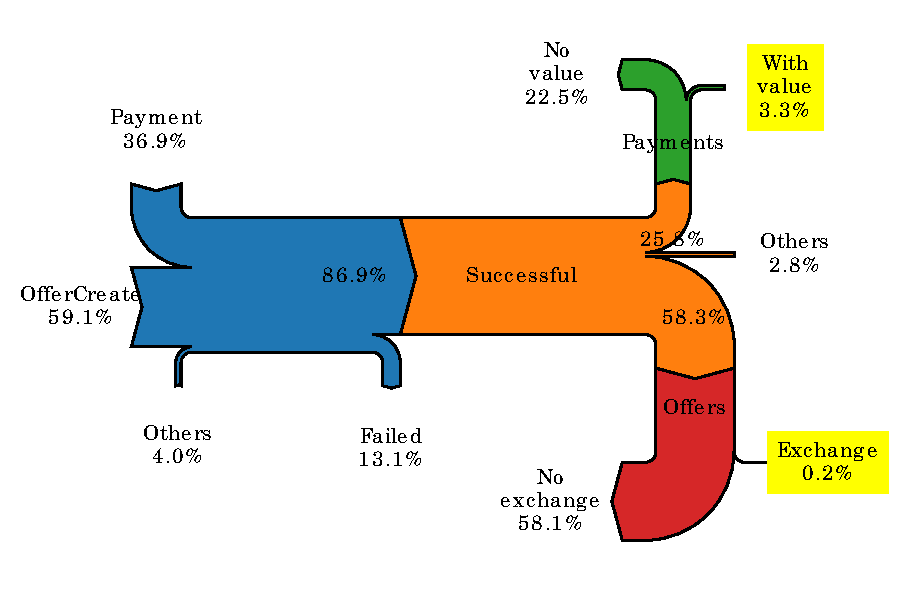
\includegraphics[
			width=\linewidth,
			trim = {0, 20, 0, 10}, clip
		]{4-transactions-security/figures/xrp-sankey.pdf}
		\caption{Observation period: \startdate to \finishdate.}
		\label{fig:xrpsakeyfull}
	\end{subfigure}
	\begin{subfigure}{\columnwidth}
		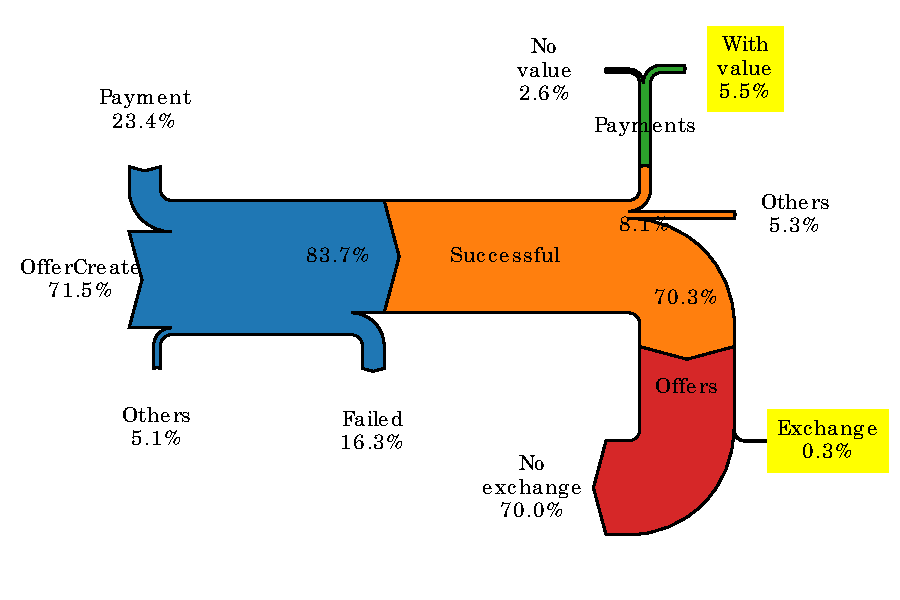
\includegraphics[
			width=\linewidth,
			trim = {0, 20, 0, 10}, clip
		]{4-transactions-security/figures/xrp-sankey3.pdf}
		\caption{Observation period: February 1, 2020, to \finishdate, during which the throughput was not polluted by systematic \texttt{Payment} spams.}
		\label{fig:xrpsakeysel}
	\end{subfigure}
	\caption[XRPL throughput by transaction type]{XRPL throughput by transaction type, success and value transferred.
		\colorbox{yellow}{Highlighted} transactions carry economic value.}
\end{figure}



Ripple suspected it to be ``an attempt to spam the ledger'' with little impact on the network.\footnote{\url{https://twitter.com/nbougalis/status/1198670099160322048}}
However, large exchanges such as Binance suffered from temporary \coin{XRP} withdrawal failures, which cited the XRP network congestion as the cause~\cite{AtoZMarkets2019}.
It remains something of a mystery how such an expensive form of ``spam'' benefited its originators.

The payment transactions from the spam did not carry any value, since they involved transferring \coin{BTC} IOU tokens unacceptable outside of the spammer's network.

To quantify true value-transferring \texttt{Payment} transactions, we retrieve the exchange rate with respect to \coin{XRP} of all the issuer-specific tokens that were transferred between \startdate and \finishdate.
Only~\empirical{12.8\%} (3.3\%/25.8\%) of all successful \texttt{Payment} transactions involve tokens with a positive \coin{XRP} rate (\autoref{fig:xrpsakeyfull}).

To obtain a picture of throughput usage uncontaminated by systematic spam, we re-examine the transaction data from February 1, 2020, to \finishdate. During this period, 67.9\% successful \texttt{Payment} transactions led to value transfer (\autoref{fig:xrpsakeysel}). Nevertheless, the value-carrying share of total throughput remains under \empirical{6\%}, since successful \texttt{Payment} transactions only account for a small fraction (\empirical{8.1\%}) of the overall traffic and the majority (\empirical{97.9\%}) of \texttt{OfferCreate} transactions eventually becomes void.


% We discover that merely~\empirical{0.2\%} of successfully created offers are fulfilled to some extent (\autoref{fig:xrpsakey}).


% which account for~\empirical{46\%} and~\empirical{50\%} of the total throughput, respectively (\autoref{fig:xrpsakey}).

% In fact, only~\empirical{1 in~19} successful \texttt{Payment} transactions involve the transfer of valuable tokens (\autoref{fig:xrpsakey}).
% All in all,~\empirical{2.3\%} of transnational throughput on the XRP ledger appears to carry economic value.

% and only~\empirical{2\%} of the transactions in the observed throughput involves actual value transfers.


In \autoref{fig:xrpcf}, we show the top senders and receivers of value-carrying \texttt{Payment} transactions, as well as the most popular currencies being transferred.
To cluster accounts, we rely on usernames as the identifier, as one entity can have multiple addresses under a given user name (e.g. \texttt{Binance}, \texttt{Coinbase}).
For accounts with no registered username, we use their parent's username, if available, plus the suffix ``descendant'' as their identifier.

As one might expect, \coin{XRP} is by far the most used currency on the ledger in terms of payment volume:~\empirical{125 billion} \coin{XRP} for seven months, or~\empirical{586 million} \coin{XRP} per day.
% The calculation aligns with the~24-hour \coin{XRP} payment volume self-reported by Ripple.\footnote{On May~31,~2020, Ripple reported~\empirical{378 million} of \coin{XRP} payment volume \cite{XRPCharts}.}

The top~10 senders cover~\empirical{53\%} of this volume, while the top~10 receivers are the beneficiaries of~\empirical{50\%} of the volume.
Payments from Ripple alone account for \empirical{7\%~(9 billion \coin{XRP})} of the \coin{XRP} volume, largely due to transactions associated with the monthly release of one billion \coin{XRP} from escrows.
While the \coin{XRP} release itself is captured through \texttt{EscrowCreate} transactions,~90\% of the released funds were unused and returned to escrows for future release~\cite{TeamRipple} through \texttt{Payment} transactions.
All other top accounts presented are held either by exchanges, or, in rare cases, by accounts that were opened by an exchange.
\texttt{Binance} appears to be the most avid \coin{XRP} user, sending~\empirical{15.2 billion} and receiving~\empirical{14.5 billion} \coin{XRP} during the observation period.

The most popular IOU tokens for fiat currencies include \coin{USD}, \coin{EUR} and \coin{CNY} (\autoref{fig:xrpcf}).
%While the ledger witnessed inter-account movements of~\empirical{2.3} billion \coin{USD},~\empirical{2.8} billion \coin{EUR} and~\empirical{43} million \coin{CNY}, only a small fraction of the corresponding tokens have value. 
Specifically,~\empirical{328} million \coin{USD},~\empirical{8} million \coin{EUR} and~\empirical{19} million \coin{CNY} issued had positive exchange rates against \coin{XRP}.
The average on-ledger exchange rates of those three fiat currency tokens, irrespective of their issuers, were~\empirical{5.4} \coin{XRP}/\coin{USD},~\empirical{5.5} \coin{XRP}/\coin{EUR} and~~\empirical{0.7} \coin{XRP}/\coin{CNY}, largely in accordance with the off-ledger exchange rates.\footnote{\url{https://finance.yahoo.com/}}
%This leads to an aggregate trading volume of~\empirical{843} million,~\empirical{19} million and~\empirical{10} million \coin{XRP} for \coin{USD}, \coin{EUR}, and \coin{CNY}, respectively, during the observation period.




\begin{figure}[tbp]
	\centering
	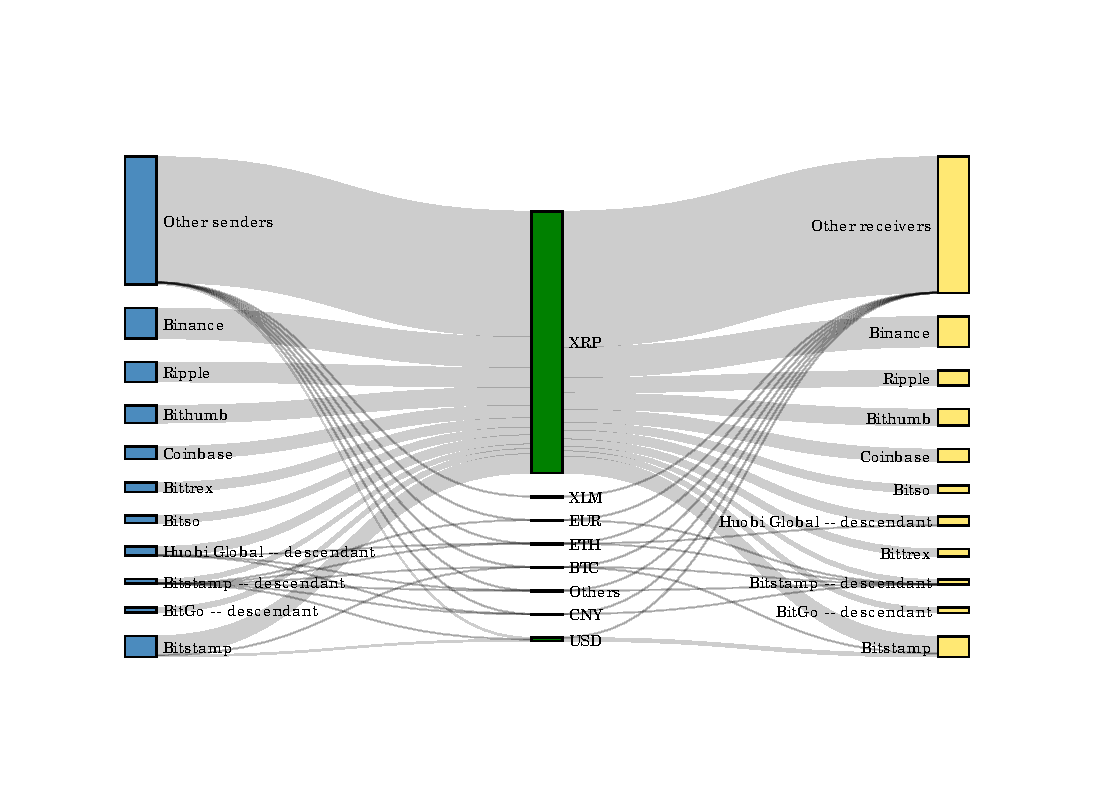
\includegraphics[width=\linewidth,
		trim = {60, 50, 62, 50}, clip]{4-transactions-security/figures/xrp-cashflow}
	\tiny{
		\textcolor{dkblue}{$\blacksquare$} Sender
		\qquad
		\textcolor{dkgreen}{$\blacksquare$} Currency
		\qquad
		\textcolor{dkyellow}{$\blacksquare$} Receiver
	}
	\caption[Value flow on the XRP ledger between \startdate and \finishdate]{Value flow on the XRP ledger between \startdate and \finishdate. The bandwidth of each flow represents the magnitude of aggregate value transferred denominated in \coin{XRP}. Only \texttt{Payment} transactions are included.}
	\label{fig:xrpcf}
\end{figure}

\point{Fulfilled offers with zero-value tokens}
% !!! https://data.ripple.com/v2/exchanges/XLM+rsdMbYxHmYswHCg1V6vBsnxmHuCjpn6SC4/XRP?start=2020-05-01T00:00:00Z&end=2019-10-01T00:00:00Z
We found a series of conspicuous payment transactions with the aggregate transfer of \empirical{360,222} \coin{BTC} IOU, issued by \xrpaddr{rKRNtZzfrkTwE4ggqXbmfgoy57RBJYS7TS}, an account activated by Liquid (\href{https://www.liquid.com/}{liquid.com}), from the issuer itself to \xrpaddr{rMyronEjVcAdqUvhzx4MaBDwBPSPCrDHYm}, an account activated by uphold (\href{https://uphold.com/}{uphold.com}).
The \coin{BTC} IOU token was exchanged at \empirical{30,500} \coin{XRP}, resulting in a valuation of \empirical{11} billion \coin{XRP} of those payments. We examine the legitimacy of the exchange rates in the next step.


The issuer is not the only factor behind the value of an IOU token.
Even IOU tokens for the same currency from the same issuer can at times exhibit vastly different rates.
\autoref{fig:xchangetime} shows an example where the \coin{BTC} IOU from the same issuer \xrpaddr{rKRNtZzfrkTwE4ggqXbmfgoy57RBJYS7TS} was traded at~\empirical{30,500} \coin{XRP} in December~2019 but then declined to~0.1~\coin{XRP} within a month.

The three exchange instances in \autoref{fig:xchangeissuer} were \texttt{OfferCreate} transactions where the initiator intended to sell \coin{BTC} ICO for \coin{XRP}.
We discover that all three offers were filled by the same account \xrpaddr{rMyronEjVcAdqUvhzx4MaBDwBPSPCrDHYm}, who received the aforementioned \coin{BTC} IOU tokens directly from the issuer's account.
Additional evidence on social media reveals that the IOU issuer's account is held by someone named \texttt{Myrone Bagalay}.\footnote{See \url{https://youtu.be/gVoyCEPvO30} and \url{https://www.twipu.com/MyroneBagalay/tweet/1161288087386894341}}
It becomes obvious that the offer taker's address, starting with \texttt{rMyronE}, must belong to the same person.

By tracing the transaction history of the concerned accounts, we notice that the two offer creators' accounts received their initial \coin{BTC} IOU tokens through payments from the offer taker.
Furthermore, one offer creator's account, \xrpaddr{rU6m5F9c1eWGKBdLMy1evRwk34HuVc18Wg}, was activated by the offer taker's account.
Now we can safely assume that all the accounts involved are controlled by that \texttt{Myrone Bagalay}, who issued \coin{BTC} IOU tokens and traded them at arbitrarily determined rates with himself.

What \texttt{Myrone Bagalay} did is completely legitimate within the confines of XRPL.
One of the key features of the ledger is the flexibility to establish a closed economy with a limited number of mutually-trusting users who can exchange self-defined assets that are not necessarily acknowledged outside the system.
However, this makes it challenging to gauge the true value transfer on XRPL since an IOU token's price---which we proxy by its exchange rate against \coin{XRP}---can be easily inflated or deflated.

Additionally, privately-issued IOU tokens that are never exchanged on the ledger, while seemingly worthless, might be valuable to their transactors after all, should they reach an agreement on those tokens' value of the ledger. However, there is no easy way to assess such value, and we leave the analysis of IOUs to future work.

\point{Summary}
In summary, the throughput on XRPL during our observation period appeared to be fraught with zero-value transactions.
We learned that both transaction volume and token value on XRPL are highly manipulable.
One must thus fully understand the underlying measurement approach to correctly interpret the resultant statistics.
